% =========================================================
\section{Mechanism: Address Translation}
% =========================================================

\begin{frame}{Address Translation}
    \begin{itemize}
        \item Memory virtualization follows the same general idea as
              \textbf{limited direct execution}.
        \item The program runs directly on the hardware whenever possible.
        \item Hardware support provides:
        \begin{itemize}
            \item \textbf{efficiency} in address translation;
            \item \textbf{control} over accessible memory;
            \item \textbf{protection} among processes and the OS.
        \end{itemize}
        \item Virtual memory should also provide flexibility in how
              applications use their address spaces.
    \end{itemize}

    \begin{block}{The Crux}
        How can we efficiently and flexibly virtualize memory while
        maintaining control over application memory accesses?
    \end{block}
\end{frame}


\begin{frame}{Hardware-Based Address Translation}
    \begin{itemize}
        \item The hardware transforms each \textbf{virtual address}
              generated by a process into a \textbf{physical address}.
        \item Translation occurs on every:
        \begin{itemize}
            \item instruction fetch;
            \item load;
            \item store.
        \end{itemize}
        \item The OS configures the hardware and manages physical memory.
        \item Goal: give each process the illusion of its own private memory.
    \end{itemize}

    \begin{block}{Tip: Interposition Is Powerful}
        Hardware interposes on every memory access, transparently
        translating virtual addresses into physical addresses.
    \end{block}
\end{frame}


\begin{frame}{Initial Assumptions}
    To introduce address translation, assume that:

    \begin{itemize}
        \item the address space is placed \textbf{contiguously}
              in physical memory;
        \item the address space is smaller than physical memory;
        \item all address spaces have the same size.
    \end{itemize}

    \begin{alertblock}{}
        These simplifying assumptions will be relaxed as more
        sophisticated virtualization mechanisms are introduced.
    \end{alertblock}
\end{frame}


\begin{frame}[fragile]{A Simple Example}
    Consider:

\begin{verbatim}
void func() {
    int x = 3000;
    x = x + 3;
    ...
}
\end{verbatim}

    A possible x86 translation is:

\begin{verbatim}
128: movl 0x0(%ebx), %eax
132: addl $0x03, %eax
135: movl %eax, 0x0(%ebx)
\end{verbatim}

    \begin{itemize}
        \item Code starts around virtual address 128.
        \item Variable \texttt{x} is located at virtual address 15KB.
        \item Instruction fetches and data accesses all generate
              virtual addresses.
    \end{itemize}
\end{frame}


\begin{frame}{A Process and Its Address Space}
    \begin{columns}
        \begin{column}{0.48\textwidth}
            \begin{itemize}
                \item Address space size: 16KB.
                \item Instructions are located at addresses
                      128, 132, and 135.
                \item Variable \texttt{x} is located on the stack
                      at address 15KB.
                \item From the process's perspective, all references
                      are within its own address space.
            \end{itemize}
        \end{column}

        \begin{column}{0.49\textwidth}

        \begin{figure}
            \centering
            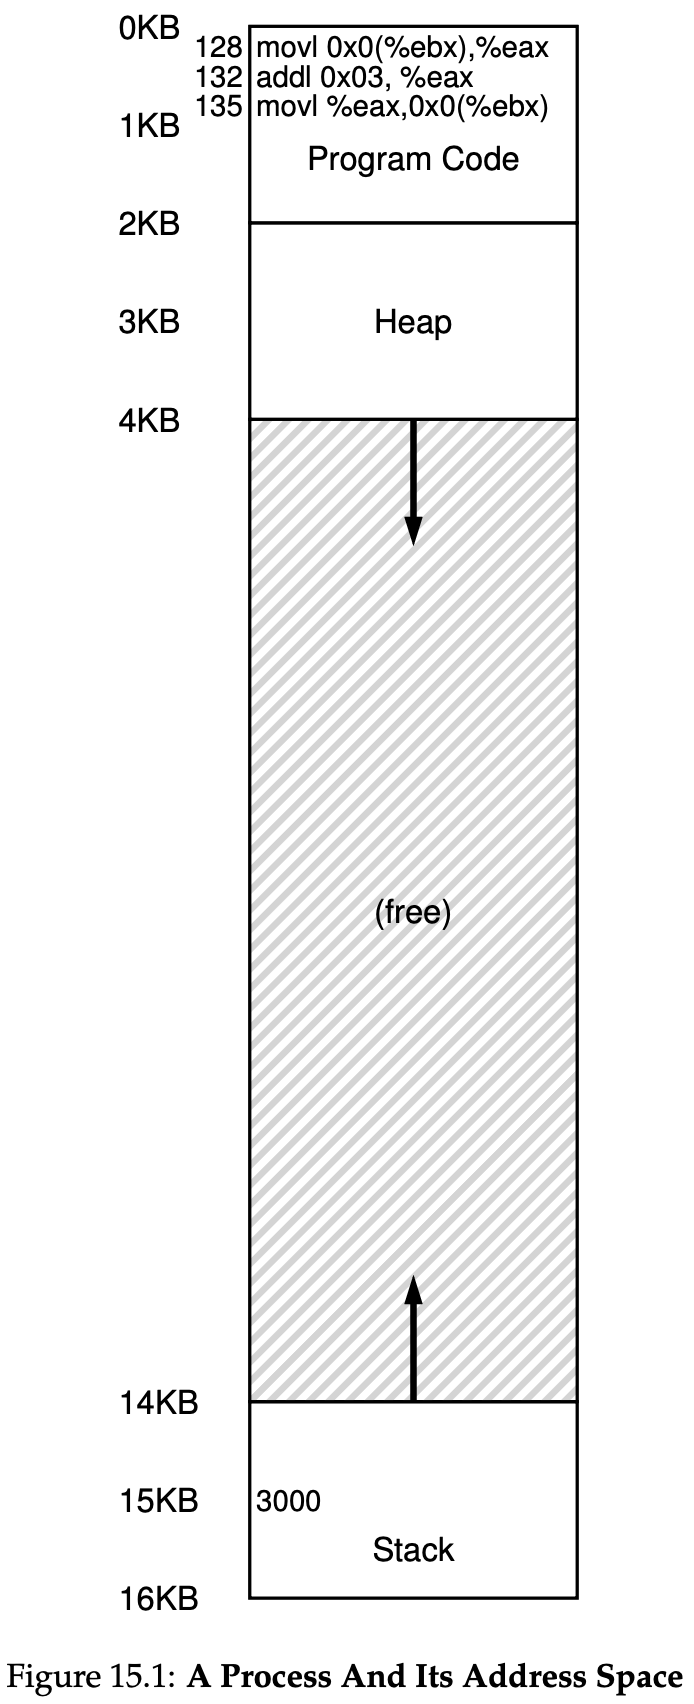
\includegraphics[width=0.5\linewidth]{figs/chapter-15/figure-15.1.png}
            \caption*{Source: chapter page 4.}
            \label{fig:figure-15.1}
        \end{figure}

        \end{column}
    \end{columns}
\end{frame}


\begin{frame}{Relocating the Process}
    \begin{columns}
        \begin{column}{0.49\textwidth}
            \begin{itemize}
                \item The process believes its address space starts at 0.
                \item The OS may place it elsewhere in physical memory.
                \item In this example, the process is relocated to
                      physical address \textbf{32KB}.
                \item Relocation must remain transparent to the process.
            \end{itemize}

            \begin{block}{Question}
                How can a virtual address space starting at 0 be mapped
                to a different physical location?
            \end{block}
        \end{column}

        \begin{column}{0.48\textwidth}

        \begin{figure}
            \centering
            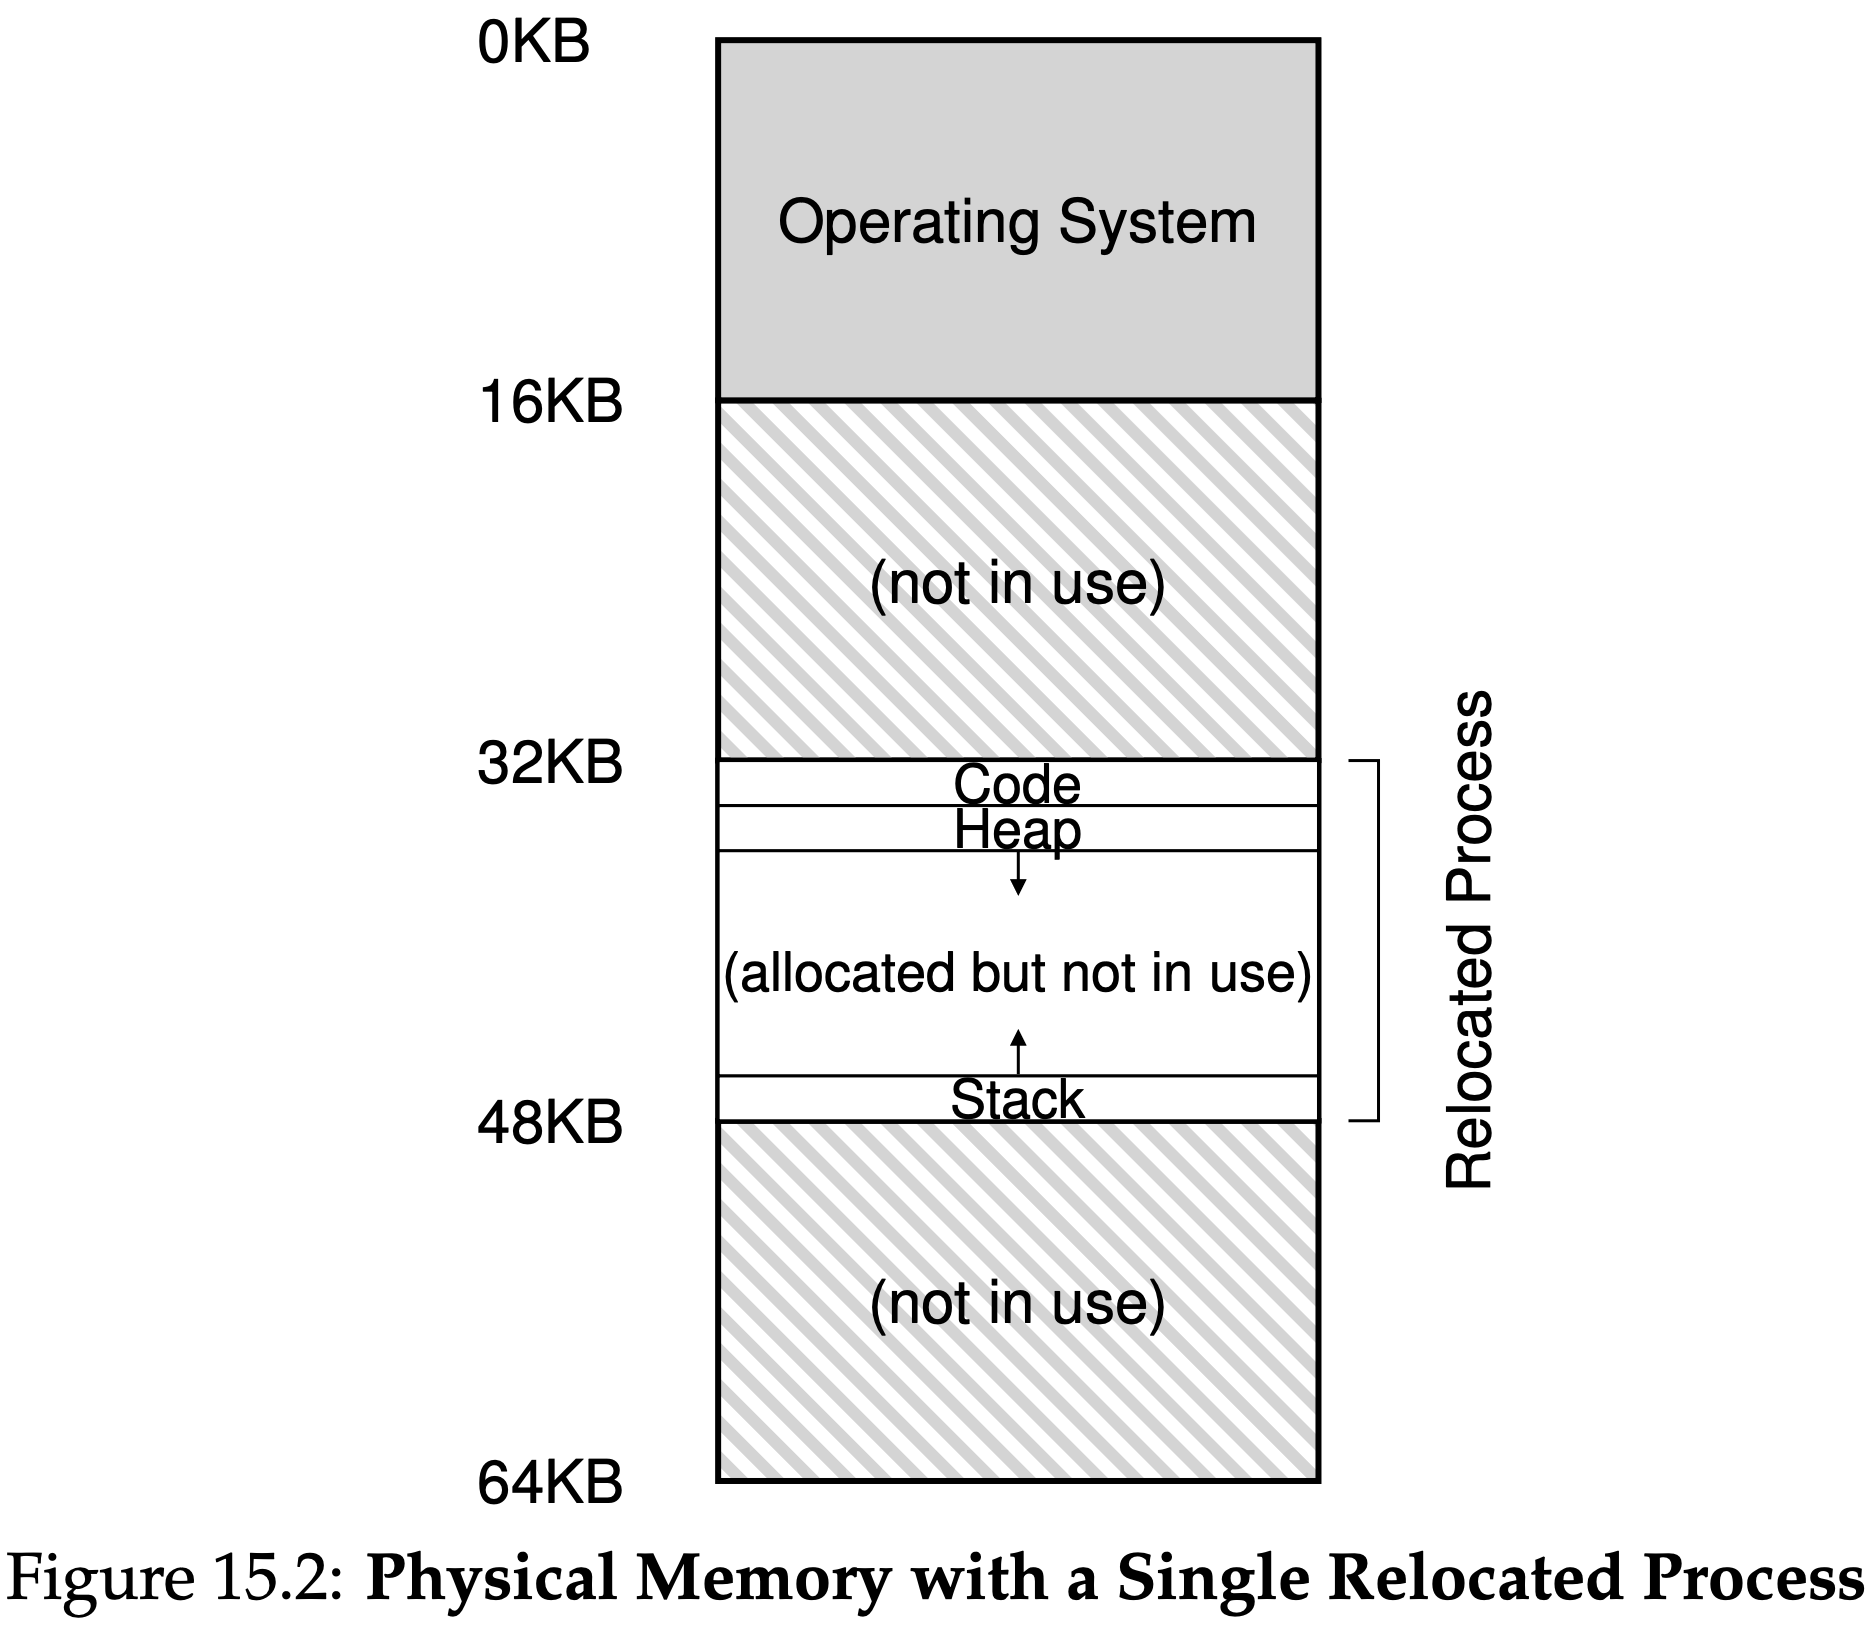
\includegraphics[width=1.1\linewidth]{figs/chapter-15/figure-15.2.png}
            \caption*{Source: chapter page 5.}
            \label{fig:figure-15.2}
        \end{figure}

        \end{column}
    \end{columns}
\end{frame}


\begin{frame}{Aside: Software-Based Relocation}
    \begin{itemize}
        \item Early systems sometimes used \textbf{static relocation}.
        \item A loader rewrote addresses before execution.
    \end{itemize}

    \begin{center}
        \texttt{movl 1000, \%eax}
        \quad $\longrightarrow$ \quad
        \texttt{movl 4000, \%eax}
    \end{center}

    \begin{itemize}
        \item Example: the process is loaded starting at physical
              address 3000.
        \item Main limitations:
        \begin{itemize}
            \item does not provide adequate protection;
            \item makes later relocation difficult.
        \end{itemize}
    \end{itemize}
\end{frame}


\begin{frame}{Dynamic Relocation: Base and Bounds}
    \begin{itemize}
        \item Dynamic relocation uses two hardware registers:
        \begin{description}
            \item[Base] physical starting address of the process;
            \item[Bounds] size or limit of the address space.
        \end{description}

        \item The program is compiled as if its address space starts at 0.
        \item The OS chooses its actual location in physical memory.
    \end{itemize}

    \begin{block}{Address Translation}
        \[
            \text{physical address}
            =
            \text{virtual address}
            +
            \text{base}
        \]
    \end{block}
\end{frame}


\begin{frame}{Example: Dynamic Relocation}
    Assume:

    \[
        \text{base} = 32\text{KB},
        \qquad
        \text{bounds} = 16\text{KB}
    \]

    \begin{itemize}
        \item Instruction fetch at virtual address 128:
        \[
            128 + 32768 = 32896
        \]

        \item Load from virtual address 15KB:
        \[
            15\text{KB} + 32\text{KB} = 47\text{KB}
        \]

        \item Translation is performed automatically by the hardware
              for every memory reference.
    \end{itemize}

    \begin{block}{Tip: Hardware-Based Dynamic Relocation}
        The base register provides relocation; the bounds register
        provides protection.
    \end{block}
\end{frame}


\begin{frame}{Bounds and Protection}
    \begin{itemize}
        \item Before accessing memory, the processor verifies that
              the virtual address is legal.
        \item If the address is:
        \begin{itemize}
            \item negative, or
            \item greater than or equal to the bounds,
        \end{itemize}
        the CPU raises an exception.

        \item The OS can then terminate the offending process.
        \item Base and bounds are maintained by the
              \textbf{Memory Management Unit (MMU)}.
    \end{itemize}

    \begin{block}{Key Idea}
        Address translation provides both \textbf{relocation}
        and \textbf{protection}.
    \end{block}
\end{frame}


\begin{frame}{Example Translations}
    Assume a 4KB address space loaded at physical address 16KB.

    \begin{center}
        \begin{tabular}{c|c}
            \textbf{Virtual Address} & \textbf{Physical Address} \\
            \hline
            0     & 16KB \\
            1KB   & 17KB \\
            3000  & 19384 \\
            4400  & Fault (out of bounds)
        \end{tabular}
    \end{center}

    \begin{itemize}
        \item A virtual address acts as an offset from the base.
        \item Out-of-bounds addresses generate an exception.
    \end{itemize}
\end{frame}


\begin{frame}{Hardware Support}
    \begin{columns}
        \begin{column}{0.48\textwidth}
            Hardware must provide:

            \begin{itemize}
                \item privileged and user modes;
                \item base/bounds registers;
                \item address translation and bounds checking;
                \item privileged instructions to update registers;
                \item exception-handler registration;
                \item ability to raise exceptions.
            \end{itemize}
        \end{column}

        \begin{column}{0.49\textwidth}

        \begin{figure}
            \centering
            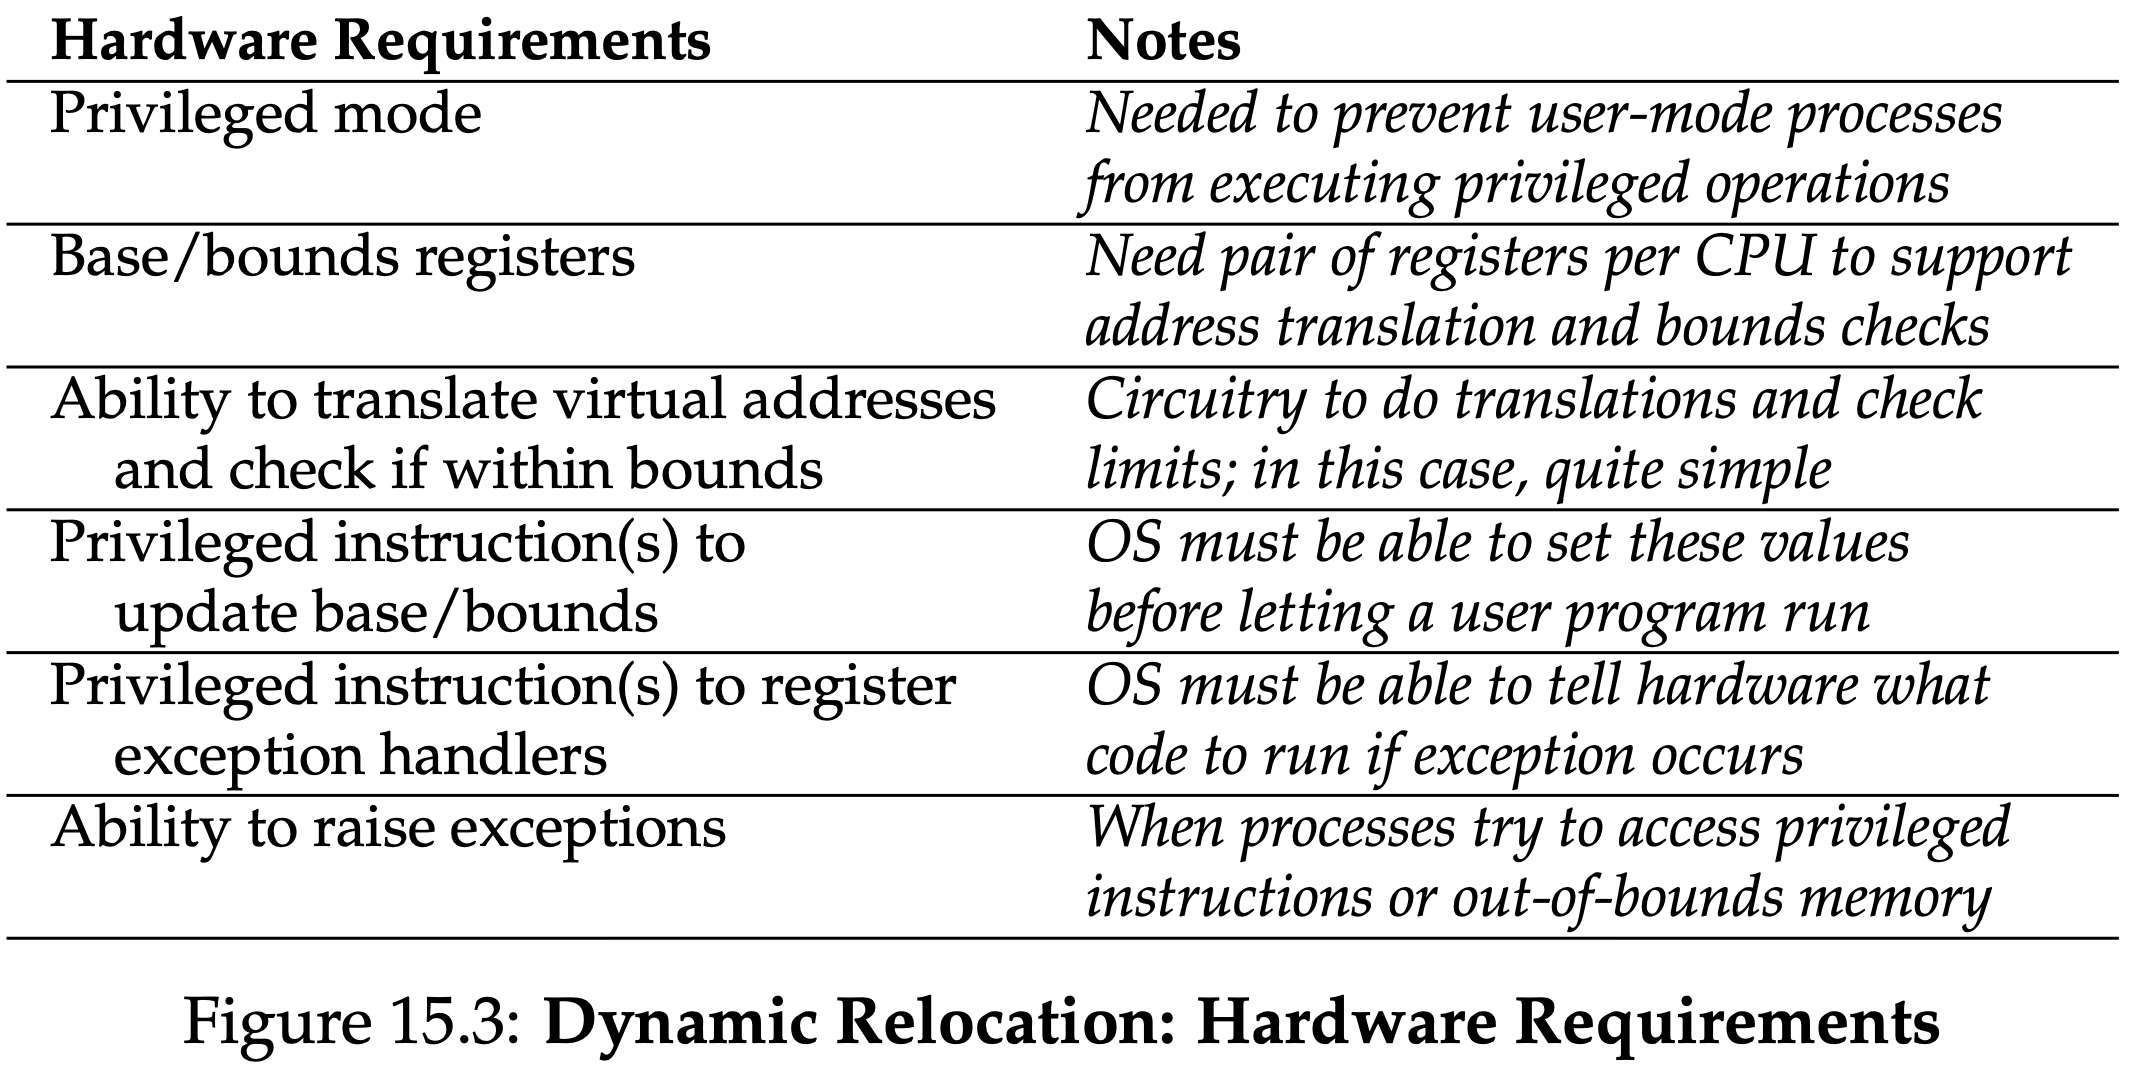
\includegraphics[width=1.1\linewidth]{figs/chapter-15/figure-15.3.png}
            \caption*{Source: chapter page 9.}
            \label{fig:figure-15.3}
        \end{figure}

        \end{column}
    \end{columns}
\end{frame}


\begin{frame}{Aside: The Free List}
    \begin{block}{Data Structure: The Free List}
        The OS must keep track of physical-memory regions
        that are currently unused.
    \end{block}

    \begin{itemize}
        \item A simple solution is a \textbf{free list}.
        \item It contains the ranges of physical memory that
              are currently available.
        \item When a process is created, the OS searches the free list
              for space.
        \item When a process terminates, its memory is returned
              to the free list.
    \end{itemize}
\end{frame}


\begin{frame}{Operating System Responsibilities}
    \begin{columns}
        \begin{column}{0.49\textwidth}
            The OS must:

            \begin{itemize}
                \item allocate memory when a process is created;
                \item reclaim memory when a process terminates;
                \item manage the free list;
                \item save and restore base/bounds during
                      context switches;
                \item install and handle exceptions.
            \end{itemize}
        \end{column}

        \begin{column}{0.48\textwidth}
        
        \begin{figure}
            \centering
            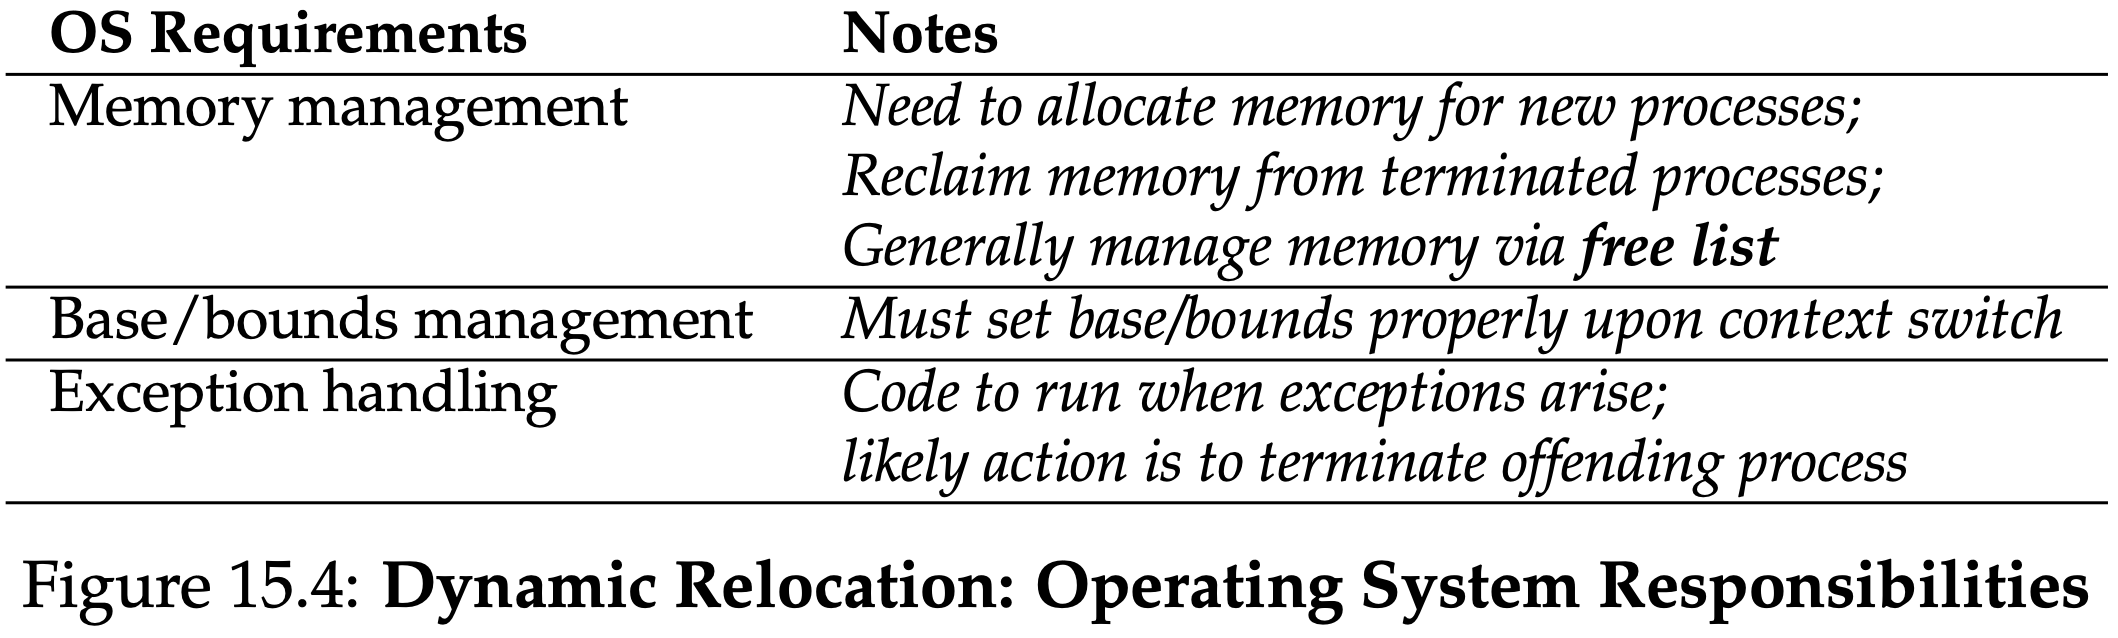
\includegraphics[width=1.1\linewidth]{figs/chapter-15/figure-15.4.png}
            \caption*{Source: chapter page 10.}
            \label{fig:figure-15.4}
        \end{figure}

        \end{column}
    \end{columns}
\end{frame}


\begin{frame}{Dynamic Relocation and Context Switching}
    \begin{itemize}
        \item Each CPU has one base/bounds pair.
        \item Different processes require different values.
        \item During a context switch, the OS:
        \begin{enumerate}
            \item saves the current base/bounds values in the
                  process structure or PCB;
            \item restores the values of the next process.
        \end{enumerate}

        \item A stopped process can even be moved to another
              physical location.
        \item The OS only needs to update its saved base value.
        \item The process remains unaware of the relocation.
    \end{itemize}
\end{frame}


\begin{frame}{Limited Direct Execution: Boot}
    \begin{columns}
        \begin{column}{0.42\textwidth}
            At boot time, the OS:
            \begin{itemize}
                \item initializes the trap table;
                \item registers exception handlers;
                \item starts the interrupt timer;
                \item initializes the process table;
                \item initializes the free list.
            \end{itemize}
        \end{column}

        \begin{column}{0.55\textwidth}

        \begin{figure}
            \centering
            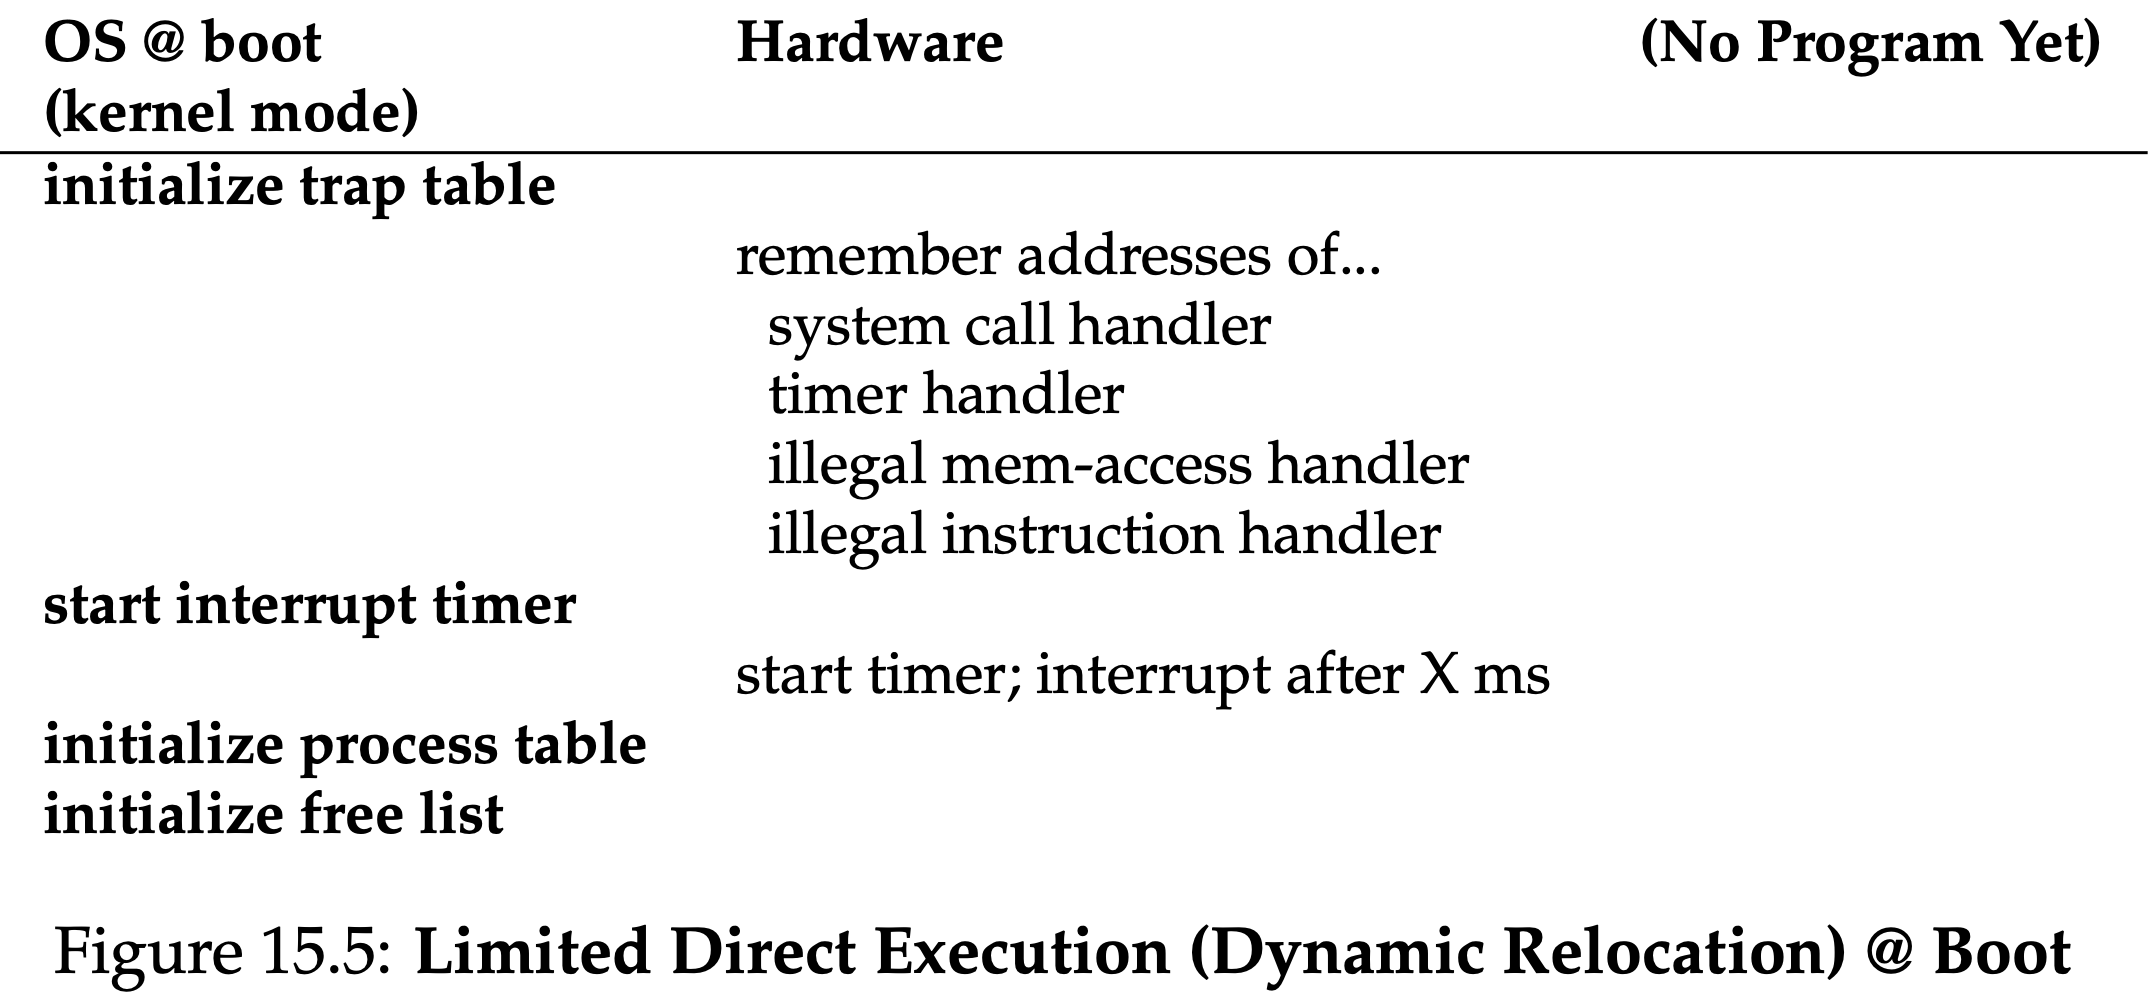
\includegraphics[width=1.1\linewidth]{figs/chapter-15/figure-15.5.png}
            \caption*{Source: chapter page 11.}
            \label{fig:figure-15.5}
        \end{figure}

        \end{column}
    \end{columns}
\end{frame}


\begin{frame}{Limited Direct Execution: Runtime}
    \begin{columns}
        \begin{column}{0.40\textwidth}
            \begin{itemize}
                \item OS configures base/bounds.
                \item Process A runs directly.
                \item Hardware translates its memory accesses.
                \item A timer interrupt returns control to the OS.
                \item OS switches to Process B.
                \item An illegal access by B causes an exception.
                \item OS terminates B and reclaims its memory.
            \end{itemize}
        \end{column}

        \begin{column}{0.57\textwidth}

        \begin{figure}
            \centering
            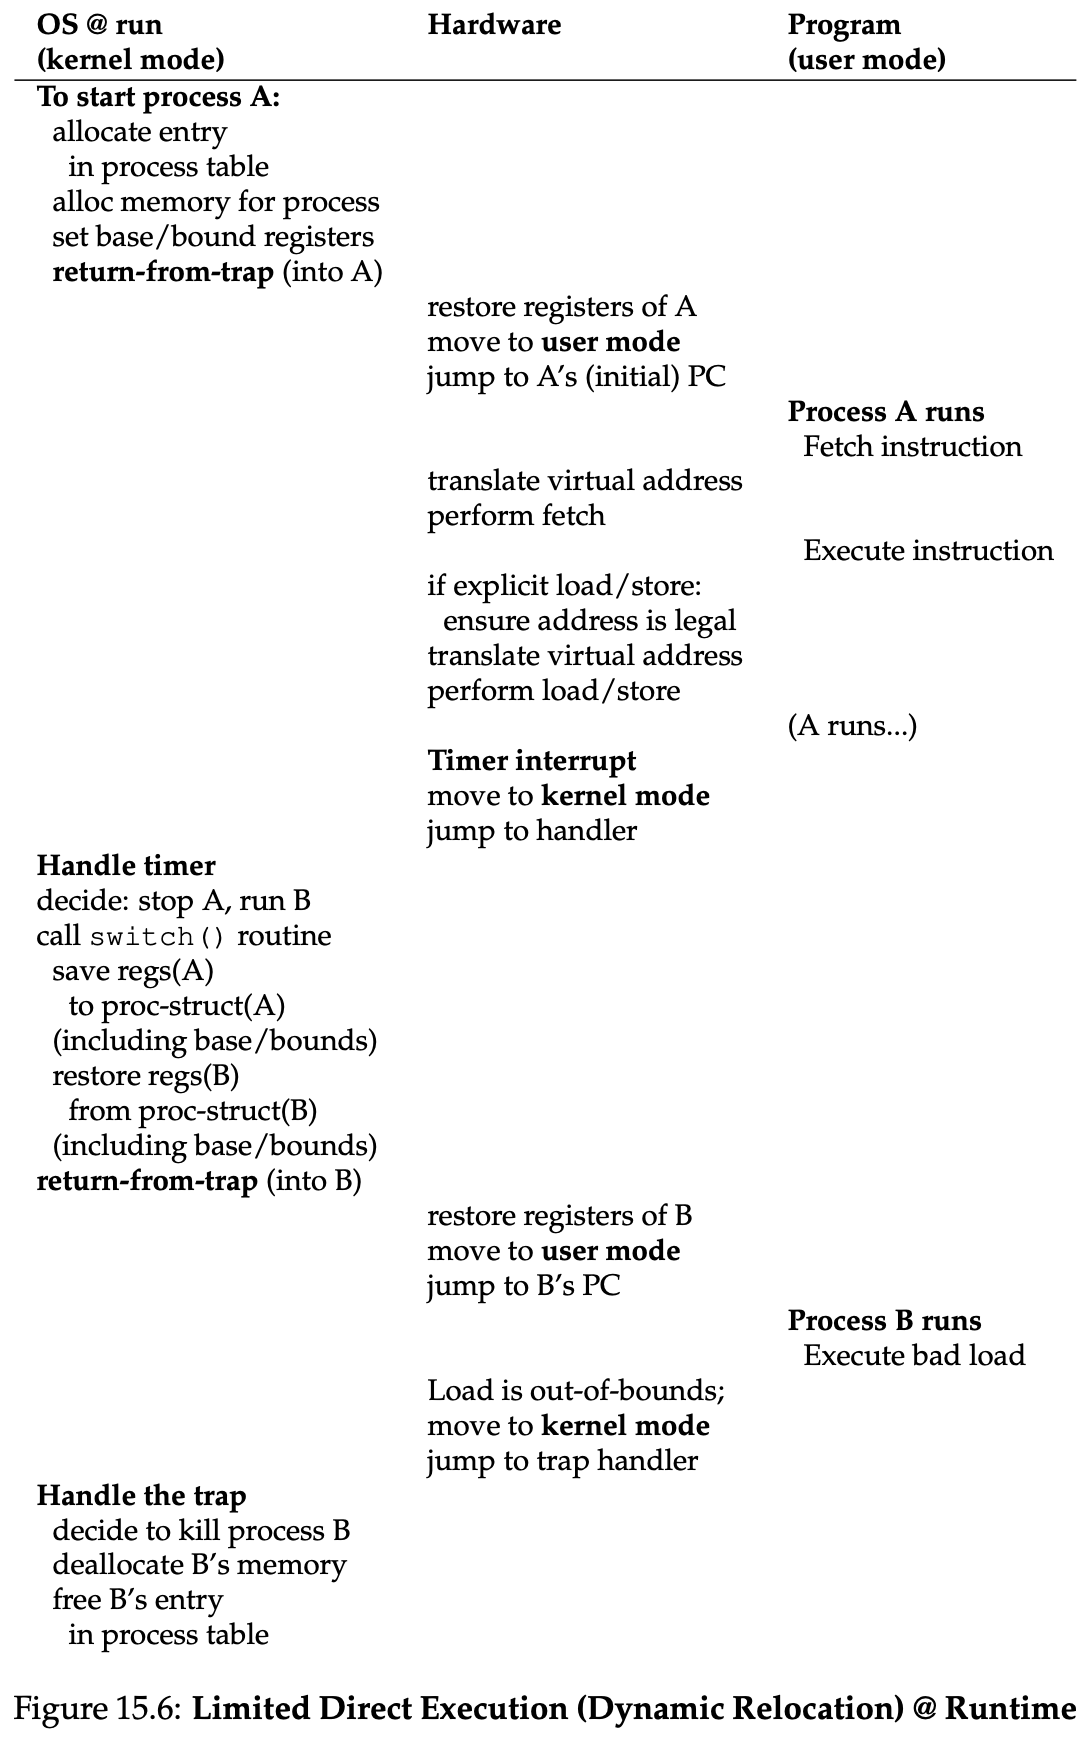
\includegraphics[width=0.6\linewidth]{figs/chapter-15/figure-15.6.png}
            \caption*{Source: chapter page 12.}
            \label{fig:figure-15.6}
        \end{figure}

        \end{column}
    \end{columns}
\end{frame}


\begin{frame}{Base and Bounds: Benefits and Limitations}
    \begin{block}{Benefits}
        \begin{itemize}
            \item Simple and efficient address translation.
            \item Transparent relocation.
            \item Protection through bounds checking.
        \end{itemize}
    \end{block}

    \begin{alertblock}{Limitation: Internal Fragmentation}
        A fixed-size address-space slot may contain large unused
        regions between the heap and stack.
    \end{alertblock}

    % Figure reference:
    % Reuse Figure 15.2 to highlight the unused region
    % inside the relocated process.
\end{frame}


\begin{frame}{Summary}
    \begin{itemize}
        \item \textbf{Address translation} extends limited direct
              execution to virtual memory.
        \item Hardware translates virtual addresses into
              physical addresses on every memory reference.
        \item \textbf{Base and bounds} provide:
        \begin{itemize}
            \item efficient dynamic relocation;
            \item transparent virtualization;
            \item memory protection.
        \end{itemize}
        \item The OS manages physical memory, context switches,
              and exceptions.
        \item Fixed-size contiguous allocation can cause
              \textbf{internal fragmentation}.
        \item A more sophisticated mechanism is therefore needed:
              \textbf{segmentation}.
    \end{itemize}
\end{frame}